\chap{A Pet Robot}\label{ch.pet}

\emph{Autonomous robots} display independent behavior that is normally
associated with living things like cats and dogs. The behavior is
achieved by \textit{feedback}: the robot will sense that something
occurs in the world and modify its behavior accordingly.

\sect{The robot obeys you}

We will program the robot to obey: the robot stays in place without
moving, but when it detects your hand in front of it, it moves towards
your hand.

{\raggedleft \hfill Program file \bu{obeys.aesl}}

There are five horizontal distance sensors on the front of the Thymio
robot and two on the rear. They are similar to the ones under Thymio
that we used in \cref{ch.moving}. Bring your hand slowly towards the
sensors; when it gets close, red lights will appear around the sensors
that detect your hands (\cref{fig.detect}).

\begin{figure}
\begin{center}
\gr{detect}{.5}
\caption{The front of the Thymio. Two sensors detect the fingers.}\label{fig.detect}
\end{center}
\end{figure}

The block \blksm{event-prox} is used to sense if something is close to a
sensor or not. In either case it causes an event to occur. The small
squares in the block (five on the front and two on the rear) are used to
specify when an event occurs. Clicking on a square changes it from gray
to white to black and back to gray. The meaning of
these colors is:

\begin{itemize}
\item \textbf{Gray}: The sensor is not used.
\item \textbf{White}: An event occurs when there is a lot of reflected
light.\label{p.proximity-colors2}
The white square has a red border
to remind you that the event will occur when the lights next to the sensor 
itself are red.
\item \textbf{Black}: An event occurs when there is little reflected
light.
\end{itemize}

If you wish an event to occur when an object is close to the sensor, use
a white square because the object will reflect a lot of light. If you
wish an event to occur when no object is close to the sensor, use a
black square because little light will be reflected.

To implement the required behavior, we need two event-actions pairs
(\cref{fig.follow-hand}). In the first pair, the center front sensor is
black and the associated action is that the motors are off. Therefore,
when the robot does not detect an object, it will not move, and it will
stop if it had been moving. In the second pair, the center front sensor
is white and the sliders of the motor block are at the top. Therefore,
when you bring your hand near the front of the robot, an event occurs
that causes both motors to run quite fast and the robot to move forward.

\begin{figure}
\begin{floatrow}
	\ffigbox
	{\caption{Moving towards your hand}\label{fig.follow-hand}}
	{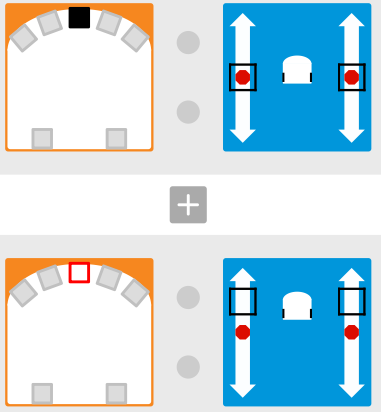
\includegraphics[width=.4\textwidth]{likes-forward}}
	\ffigbox
	{\caption{A bulldozer with tracks}\label{fig.bull}}
	{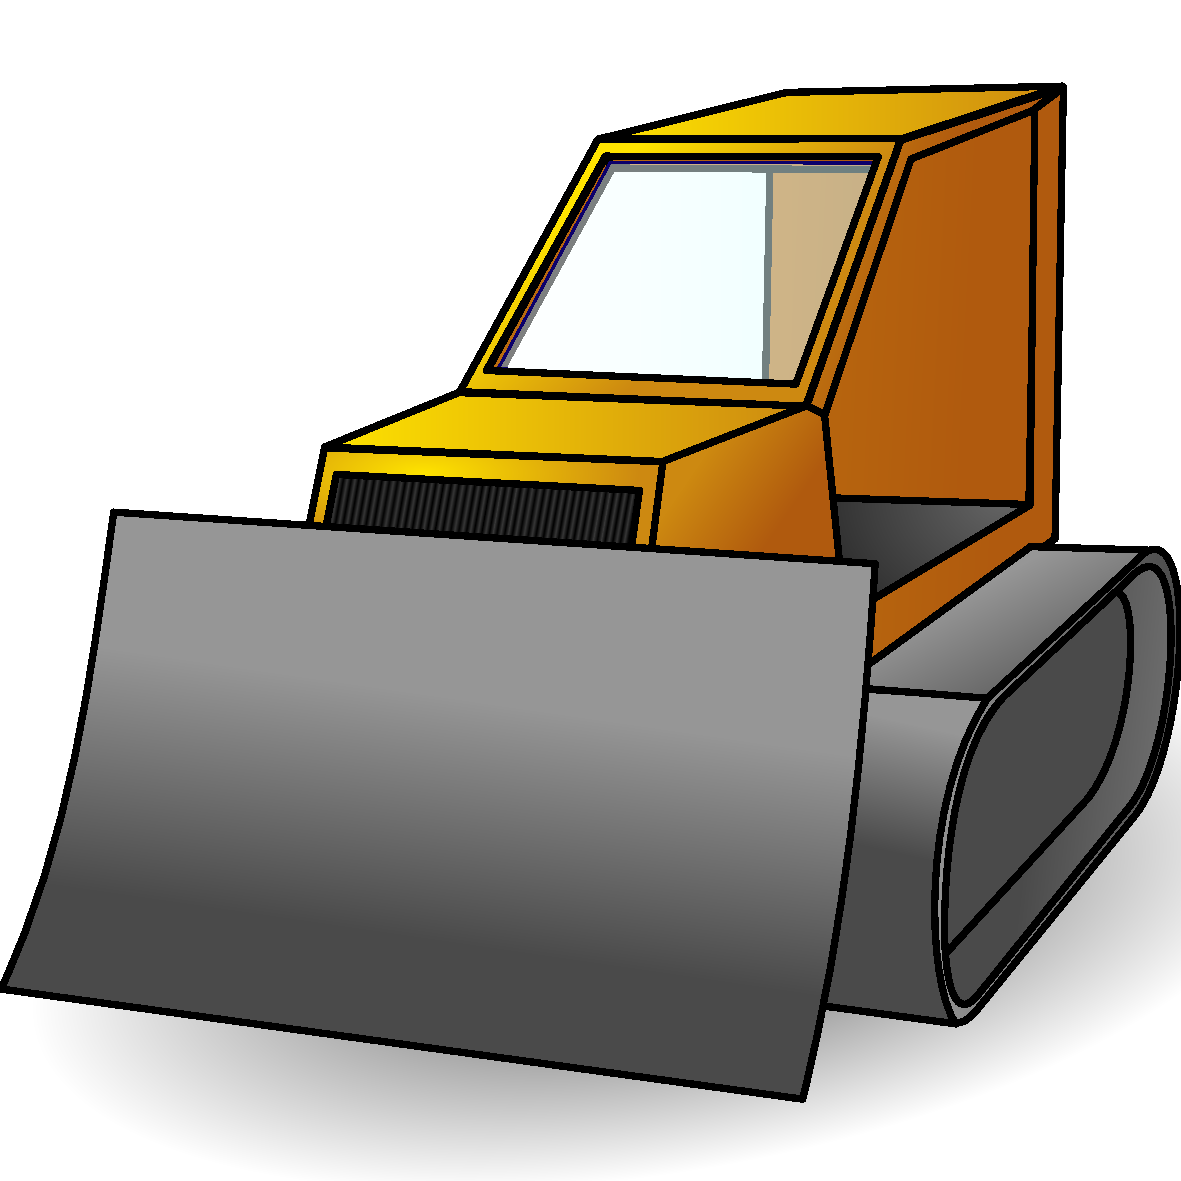
\includegraphics[width=.35\textwidth]{bulldozer}}
\end{floatrow}
\end{figure}

\sect{Steering the Thymio robot}

The Thymio robot does not have a steering wheel like a car or a
handlebar like a bicycle. So how can it turn? The robot uses
\emph{differential drive}, which is familiar from tracked vehicles like
the bulldozer (\cref{fig.bull}). Instead of turning a handlebar a
desired direction, the left and right tracks or wheels are driven by
individual motors at \emph{different} speeds. If the right track moves
faster than the left one, the vehicle turns left, and if the left track
moves faster than the right one, the vehicle turns right.

Differential drive for the Thymio robot is implemented by setting the
left and right sliders of a motor action block---and therefore the wheel
speeds---to different values. The greater the difference between the
speeds, the tighter the turn. To achieve a large difference of speeds,
drive one track forward and one track backwards. In fact, if one
track moves forward at a certain speed, while the other track moves
backwards at the same speed, the Thymio turns in place. For example, in
the motor action block \blksm{differential}, the left slider has been
set for fast speed backwards, while the right slider has been set for
fast speed forwards. The result is that the robot will turn to the left.

\newpage

Experiment with an event-actions pair such as: \blkc{turning}

Set the left and right sliders, run the program and touch the center
button; to stop the robot click on \blksm{stop}. Now you can change the
sliders and try again.

\trickbox{The small image of Thymio in the center of the motor action
block shows an animation of the movement of the robot when you move the
sliders. When the animation stops, the image shows the direction in
which the robot will move when this action block is run.}

\sect{The robot likes you}

A real pet follows you around. To make the robot follow your hand, add
two additional event-actions pairs: if the robot detects an object in
front of its left-most sensor, it turns to the left, while if it detects
an object in front of its right-most sensor, it turns to the right.
                                                       
{\raggedleft \hfill Program file \bu{likes.aesl}}

The program consists of two event-actions pairs (\cref{fig.likes}).
Experiment with the sliders on the motor action blocks.

\begin{figure}
	\subfigure[The robot likes you]{
		\label{fig.likes}
		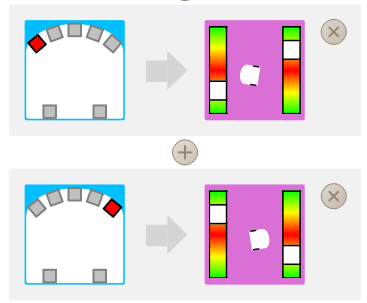
\includegraphics[width=.4\textwidth]{likes-turns}
	}
	\hfill
	\subfigure[The robot doesn't like you]{
		\label{fig.hates}
		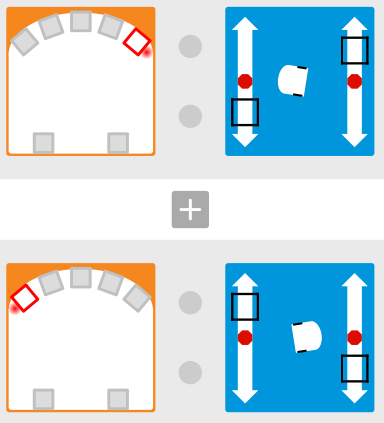
\includegraphics[width=.4\textwidth]{hates}
	}
	\caption{Programs for the pet robot}\label{fig.likes-hates}
\end{figure}

\exercisebox{\thechapter.1}{ Modify the behaviour of the robot so
that it moves forward when the program is run and stops when it
detects the edge of a table (or a strip of black tape).}

\exercisebox{\thechapter.2}{ What happens if you change the order of the
event-actions pairs that you used in the previous exercise? }

\sect{The robot doesn't like you}

Sometimes your pet may be in a bad mood and turn away from your hand.
Write a program that causes this behavior in the robot.

{\raggedleft \hfill Program file \bu{does-not-like.aesl}}

Open the program for the pet that likes you and exchange the association
of the events with the actions. Detection of an object by the left
sensor causes the robot to turn right, while detection of an object by
the right sensor causes the robot to turn left (\cref{fig.hates}).

% \begin{figure}[htb]
% \begin{center}
% \gr{hates}{0.4}
% \caption{The robot doesn't you}\label{fig.hates}
% \end{center}
% \end{figure}

\exercisebox{\thechapter.3} { The front horizontal sensors are numbered
0, 1, 2, 3, 4 from the left of the robot to its right. The rear sensors
are numbered 5 for the left one and 6 for the right one. Modify the
programs in \cref{fig.likes-hates} so that instead of
using sensors 0 and 4:
\begin{itemize}[noitemsep,nosep,leftmargin=*]
\item Use sensors 1 and 3 to turn the robot left and right, respectively.
\item Use both sensors 0 and 1 to turn the robot left and both sensors 3
and 4 to turn the robot right.
\item Add event-actions pairs for the rear sensors 5 and 6.
\end{itemize}
}

\bigskip

\trickbox{\cref{a.tech} explains how to set the sliders to
precsie motor speeds.}

\bigskip

\informationbox{Sensors in advanced mode}{In advanced mode
(\cref{ch.time}), there is a fourth mode for specifying when sensors cause
events, in addition to modes indicated by
gray, white and black. See \cref{a.tech}.}
